%%%%%%
%$Autor: Elmar Wings$
%$Projekt: $
%$Dateiname: SensorRFIDRC522.tex$
%$Beschreibung: Erläuterung des verwendeten RFID-Sensors$
%%%%%%


%\chapter{RFID}}\label{RFID-Sensor RC522}



%\begin{figure}[H]
%	\centering
%	\begin{tikzpicture}
	
%		\rfidSensor{1.0}{0}{0}{0}
%		
%		\draw[red, line width=4mm] (rcPin-MOSI) -- ++(0, -2); 
%		\draw[red, line width=0.4] (rcPin-SDA) -- ++(0, -2); 
%		
%	\end{tikzpicture}
%\end{figure}


%RFID-Reader (Radio Frequency Identification) sind zentrale Bestandteile berührungsloser Identifikationssysteme. 
%Zu einem RFID-System gehört neben dem Reader (Empfänger) immer auch ein Sender, in der Regel ist dies die Schlüsselkarte. 
%Die Kommunikation erfolgt über elektromagnetische Felder. 
%Der Reader erzeugt ein hochfrequentes Wechselfeld, das in der Antenne des Tags eine Spannung induziert und so die Schl\"usselkarte mit Energie versorgt (passive Tags). 
%
%Gleichzeitig \"uberträgt der Reader über modulierte Signale Informationen, z. B. ein Lesebefehl.
%Die Schlüsselkarte antwortet, indem sie seine Antennenschaltung ver\"andert. 
%Das Prinzip wird als „Load Modulation“ bezeichnet.
%Die daraus resultierenden \"Anderungen im elektromagnetischen Feld kann der Reader detektieren und zur\"uck in digitale Daten umwandeln.
%
%Während Systeme wie der RC522 im HF-Bereich mit induktiver Kopplung arbeiten, nutzen moderne UHF-Systeme (z. B. bei 868 MHz) elektromagnetische Wellen im Fernfeld.
%Diese ermöglichen gr\"oßere Reichweiten, erfordern jedoch spezielle Antennentechniken, da sich das Ausbreitungsverhalten mit steigender Frequenz ver\"andert. 
%Reflexionen, D\"ampfungen und Richtwirkungen nehmen zu, was den Einsatz komplexer Filter- und Verst\"arkertechnik notwendig macht.
%
%Der Reader besteht daher oft aus einem analogen Frontend zur Frequenzaufbereitung und einem digitalen Signalprozessor (DSP) zur Verarbeitung und Steuerung der Kommunikation.
%Die Wahl der Frequenz, wie beim RC522 die 13{,}56~MHz, beeinflusst die Reichweite, Kopplungsart und mögliche Anwendungen.
%RFID-Technik hat sich über die Jahre von einfachen Identifikationsl\"osungen mit geringer Reichweite zu leistungsf\"ahigen Kommunikationssystemen entwickelt. 
%RFID-Systeme finden breite Anwendung in der Logistik, Zugangskontrolle, Einzelhandel und im Gesundheitswesen. 
%Sie ermöglichen die kontaktlose Identifikation und Nachverfolgung von Waren, Personen und Tieren. 
%In Bibliotheken und Archiven erleichtern sie die Medienverwaltung, während sie in der Bauindustrie die \"Uberwachung von Werkzeugen und Ausrüstungen unterst\"utzen. 
%RFID-Technologie optimiert Prozesse und steigert die Effizienz in verschiedenen Bereichen.
%
%Für Arduino Anwendungen, die ein sicheres Identifikationsverfahren erfordern, bietet sich RFID an. Mithilfe elektromagnetischer Wellen ermöglicht es eine berührungslose Identifikation. Dieses Verfahren findet auch beim zunehmend beliebten kontaktlosen Bezahlen mit EC- oder Kreditkarten Verwendung. Ein RFID-Modul wird in der Regel mit einer RFID-Karte und einem Schlüsselanhänger geliefert. Es kommt häufig in Anwesenheitssystemen sowie anderen Anwendungen zur Identifikation von Personen oder Objekten zum Einsatz.
% \cite{Heuermann2023} \cite{AZDelivery2025}
%

%%%%%%%%%% SHAMSA  %%%%%%%%%%%%%%%%%%%%%

\chapter{RFID}
%\label{RFID-Sensor RC522}
%\chapter{Radio Frequency Identification}



\section{Allgemein}

Die RFID-Technologie ist ein Verfahren zur automatisierten und kontaktlosen Identifikation von Objekten, Personen oder Tieren. 
Der Begriff \ac{rfid} steht für \textit{Radio Frequency Identification} und wird als \enquote{Funk-Identifikation} übersetzt. 
Ein \ac{rfid}-Tag überträgt eine eindeutige Seriennummer, die für jeden Transponder individuell ist, 
wodurch auch äußerlich identische Objekte eindeutig voneinander unterschieden werden können \cite{Heuermann:2023}.

Im Verlauf dieser Dokumentation wird zur Vereinfachung ausschließlich der Begriff \enquote{Transponder} verwendet. 
Dieser umfasst sowohl klassische \ac{rfid}-Schlüsselanhänger als auch kontaktlose Chipkarten, 
da beide auf demselben physikalischen Prinzip basieren und nach dem internationalen Standard ISO/IEC~14443~A arbeiten.

Grundsätzlich wird zwischen verschiedenen Transpondertypen unterschieden, 
die sich hinsichtlich ihrer Energieversorgung und Kommunikationsreichweite unterscheiden. 
Diese Kategorien – passive, semi-passive und aktive Transponder – werden im weiteren Verlauf der Arbeit ausführlich beschrieben (vgl. Abschnitt~\ref{subsec:transpondertypen}.



Die \ac{rfid}-Technologie ist ein Verfahren zur automatisierten und kontaktlosen Identifikation von Objekten, Personen oder Tieren. 
Der Begriff \ac{rfid} steht für Radio Frequency Identification und wird als „Funk-Identifikation“ übersetzt. 
Im Gegensatz zu einem Barcode, der in der Regel nur die Produktart kennzeichnet, überträgt ein \ac{rfid}-Tag eine eindeutige Seriennummer, welche jeder Tag individuell besitzt.
Damit können auch äußerlich identische Objekte voneinander unterschieden werden \cite{Heuermann:2023}. 


\subsection{Aufbau und Funktionsweise}

Ein \ac{rfid}-System besteht im Wesentlichen aus zwei Komponenten:

\begin{itemize}
	\item \textbf{Reader (Lesegerät)}: erzeugt das elektromagnetische Feld, versorgt die Transponder mit Energie und übernimmt die Steuerung des Datenaustauschs. 
	Er besteht aus zwei Teilen: 
	\begin{itemize}
		\item einem digitalen Teil, der die Signale verarbeitet und die empfangenen Antworten wieder in Daten umwandelt (Demodulation),
		\item sowie einem analogen Teil, der für die Erzeugung, Verstärkung und Filterung der Funksignale zuständig ist. 
	\end{itemize}
	Stationäre oder mobile Reader können die erfassten Informationen, wie zum Beispiel die eindeutige Seriennummer \ac{uid} oder Zeitstempel, direkt speichern oder an eine Datenbank weitergeben. 
	\item \textbf{Transponder (Tag)}: kleine Mikrochips mit Antenne, die Informationen speichern und bei Anfragen des Readers übermitteln \cite{Heuermann:2023}. 
\end{itemize}



\subsection{Systemkommunikation}

Die Kommunikation zwischen Reader und Transponder erfolgt über ein elektromagnetisches Feld. 
Dieses Feld wird durch eine Spule im Reader erzeugt, die von einem hochfrequenten Wechselstrom durchflossen wird. 
Dadurch entsteht ein sich ständig veränderndes Magnetfeld, das sich um die Antenne des Readers ausbreitet und vom Transponder aufgenommen werden kann \cite{Conrad:2024a}. 
Bei \ac{hf}-Systemen mit 13{,}56~MHz funktioniert die Energieübertragung ähnlich wie bei einem Transformator: 
Das Magnetfeld des Readers regt die Spule im Tag an und versorgt den integrierten Schaltkreis mit Energie. 
In \ac{uhf}-Systemen werden dagegen Funkwellen genutzt, die sich wie Radiosignale über größere Entfernungen ausbreiten können \cite{Rieback:2006}.  

Passive Transponder besitzen keine eigene Energiequelle, sondern nutzen das elektromagnetische Wechselfeld des Readers. 
In der Antenne des Tags wird durch Induktion eine Spannung erzeugt, die in Gleichstrom umgewandelt wird und so die Versorgung des Chips übernimmt \cite{Conrad:2024a}. 
Eine Darstellung des inneren Aufbaus und der Funktionsweise passiver Transponder erfolgt in Abschnitt \ref{subsec:transponderfunktion}, ergänzt durch eine Abbildung zur Veranschaulichung (vgl. Abbildung~\ref{fig:rfid-tag}). 




Die Datenübertragung basiert auf dem Prinzip der Load Modulation: 
Der Reader sendet modulierte Befehle, während der Tag durch gezielte Änderungen seiner Antennenschaltung das Feld beeinflusst. 
Diese Änderungen führen zu messbaren Schwankungen im Signal, die vom Reader in digitale Informationen umgesetzt werden. 
Dabei handelt es sich beispielsweise um die eindeutige Seriennummer \ac{uid} des Transponders, um gespeicherte Produktinformationen wie Artikelnummern oder Barcodes, um Authentifizierungsdaten oder um weitere im Tag hinterlegte Informationen \cite{Heuermann:2023,Conrad:2024a}.

\subsection{Arten von Transpondern}\label{transpondertypen}

Transponder lassen sich nach ihrer Energieversorgung unterscheiden:

\begin{itemize}
	
	
	\item \textbf{Passive Tags}: werden ausschließlich durch das elektromagnetische Feld des Readers mit Energie versorgt und enthalten mindestens eine eindeutige Kennung, beispielsweise einen \ac{epc} oder eine \ac{tid}.
 
	\item \textbf{Semi-passive Tags}: besitzen eine kleine Batterie zur Versorgung der internen Logik, nutzen jedoch weiterhin das Feld des Readers für die Kommunikation.  
	\item \textbf{Aktive Tags}: verfügen über eine eigene Stromquelle, erreichen Reichweiten von über 100 Metern und können auch selbständig Signale aussenden \cite{Conrad:2024a}. 
	
	
\end{itemize}


Der \ac{epc} ist ein standardisiertes Datenformat, das zur eindeutigen Kennzeichnung von Produkten dient und vor allem in der Logistik eingesetzt wird.
Der \ac{tid} ist dagegen die vom Hersteller fest vergebene und unveränderliche Seriennummer des RFID-Chips. 
Im Unterschied zur \ac{uid}, die ebenfalls eine eindeutige Nummer darstellt, aber bei manchen Chiptypen veränderbar ist, bleibt der \ac{tid} stets hardwareseitig festgeschrieben.

\subsection{Frequenzbereiche und Reichweiten}

Die Reichweite und die Übertragungsgeschwindigkeit eines \ac{rfid}-Systems hängen wesentlich vom genutzten Frequenzbereich ab. 
Man unterscheidet dabei mehrere Hauptbereiche:

\begin{itemize}
	\item \textbf{\ac{lf}} (125–134 kHz): Reichweite bis etwa 30 cm, häufig eingesetzt in Zugangskontrollsystemen oder zur Tierkennzeichnung. 
	\item \textbf{\ac{hf}} (13,56 MHz): Reichweite bis etwa 1 m, verwendet in \ac{nfc}-Anwendungen, Bibliotheken, Smartcards und beim kontaktlosen Bezahlen. 
	\item \textbf{\ac{uhf}} (860–960 MHz): Reichweiten bis etwa 30 m bei passiven und über 100 m bei aktiven Transpondern, vor allem in Logistik und Warenverfolgung.
	\item \textbf{\ac{shf}} (2,45 GHz): Reichweiten bis etwa 10 m, typischer Einsatz in Mautsystemen oder industriellen Anwendungen \cite{Heuermann:2023,Conrad:2024a}. 
\end{itemize}

\subsection{Internationale Unterschiede}

Die zugelassenen Frequenzbereiche für RFID sind nicht weltweit einheitlich geregelt. 
Besonders im \ac{uhf}-Bereich bestehen Abweichungen: 
In Europa ist das Band von 865–868~MHz vorgesehen, während in Amerika 902–928~MHz genutzt wird. 
Diese Unterschiede sind insbesondere für Anwendungen in der Logistik und industriellen Kennzeichnung relevant, da \ac{uhf}-Systeme dort weit verbreitet sind. 
Die Bereiche für \ac{lf}, \ac{hf} und \ac{shf}  sind hingegen international weitgehend harmonisiert \cite{finkenzeller:2019}.  

Die regulatorischen Vorgaben stammen in Europa von der \ac{etsi} und in Amerika von der \ac{fcc}. 
Geräte, die für den amerikanischen Markt ausgelegt sind, können in Europa oft nicht ohne Anpassung betrieben werden. 
Ursache sind vor allem die unterschiedlichen Frequenzbänder im \ac{uhf}-Bereich sowie Unterschiede bei der erlaubten Sendeleistung \cite{finkenzeller:2019}.  

Die in der RFID-Technologie genutzten Frequenzbereiche und deren internationale Unterschiede sind in Tabelle~\ref{tab:TabelleFrequenzbereiche} dargestellt. 
Die Übersicht zeigt zudem die typischen Anwendungsfelder der jeweiligen Bereiche \cite{finkenzeller:2019}.

\begin{table}[H]
	\caption{RFID-Frequenzbereiche und internationale Unterschiede \cite{finkenzeller:2019}}
	\label{tab:TabelleFrequenzbereiche}
	\begin{tabular}{|l|l|l|l|}
		\hline
		\textbf{Frequenzbereich} & \textbf{Europa} & \textbf{Amerika} & \textbf{Typische Anwendung} \\ \hline
		\ac{lf} & 125–134~kHz & 125–134~kHz & Zugangssysteme \\ \hline
		\ac{hf} & 13{,}56~MHz & 13{,}56~MHz & \ac{nfc}, kontaktloses Bezahlen \\ \hline
		\ac{uhf} & 865–868~MHz & 902–928~MHz & Logistik, Lagerhaltung \\ \hline
		\ac{shf} & 2{,}45~GHz & 2{,}45~GHz & Mautsysteme, Industrie \\ \hline
	\end{tabular}
\end{table}










\subsection{Entwicklung und Anwendungen}

Die Ursprünge von \ac{rfid} liegen im Zweiten Weltkrieg, als Funkwellen im sogenannten \ac{iff} zur Unterscheidung von Flugzeugen eingesetzt wurden. 
Seitdem wurde die Technologie kontinuierlich weiterentwickelt und findet heute in zahlreichen Bereichen Anwendung: 

\begin{itemize}
	\item Logistik und Handel: Nachverfolgung von Waren und Paletten, Warensicherung, 
	\item Zugangskontrolle: Gebäude, Labore, Fahrzeuge, 
	\item Gesundheitswesen: Patienten- und Geräteidentifikation, 
	\item Bibliotheken und Archive: automatische Medienverwaltung, 
	\item Alltag: elektronische Ausweise, Reisepässe, kontaktloses Bezahlen \cite{Rieback:2006,Liu:2024}. 
\end{itemize}

%\subsection*{Sicherheit und Datenschutz}
%
%Mit der weiten Verbreitung von \ac{rfid}-Systemen ergeben sich Herausforderungen im Bereich Sicherheit und Privatsphäre. 
%Mögliche Angriffe sind unautorisiertes Auslesen Skimming, Klonen von Tags, Mithören (Eavesdropping) oder Relay-Angriffe. 
%Zum Schutz werden verschiedene Verfahren eingesetzt, darunter Kill- oder Sleep-Kommandos, Challenge-Response-Authentifizierung, Verschlüsselung oder Blocking-Tags. 
%Einfache passive Tags haben dabei Einschränkungen, da sie nur über begrenzte Rechenressourcen verfügen \cite{Mitrokotsa:2010,Aragones2007}. 



\subsection{Sicherheit und Datenschutz}

Die Nutzung von \ac{rfid}-Systemen bringt neben funktionalen Vorteilen auch verschiedene sicherheitstechnische und datenschutzrechtliche Herausforderungen mit sich. 
Ein wesentliches Merkmal dieser Technologie ist die drahtlose Kommunikation über Funk. 
Dadurch können Daten nicht nur von autorisierten Lesegeräten, sondern potenziell auch von Angreifern erfasst werden. 
Besonders problematisch ist, dass viele einfache Transponder nur sehr begrenzte Rechenleistung haben und daher keine aufwändigen Sicherheitsmechanismen unterstützen. 
Dies führt dazu, dass grundlegende Sicherheitsmechanismen wie starke Verschlüsselung, Zugriffskontrolllisten oder dynamische Authentifizierung in kostengünstigen Systemen oft fehlen \cite{Mitrokotsa:2010,Aragones:2007}.

Zu den typischen Angriffsszenarien gehören:
\begin{itemize}
	\item \textbf{Skimming}: unautorisiertes Auslesen eines Transponders ohne Wissen des Besitzers, auch aus größerer Entfernung als vorgesehen.
	\item \textbf{Klonen}: Anfertigen einer Kopie eines gültigen Transponders, um diesen für unbefugte Zwecke zu nutzen.
	\item \textbf{Mithören (Eavesdropping)}: passives Abhören der Kommunikation zwischen Transponder und Lesegerät durch ein drittes Gerät, das im Empfangsbereich positioniert ist. Da viele Protokolle unverschlüsselt arbeiten, können eindeutige Identifikatoren oder gespeicherte Daten mitgelesen werden.
	\item \textbf{Relay-Angriffe}: Weiterleitung der Kommunikation zwischen Transponder und Lesegerät über größere Entfernungen. Dabei agieren Angreifer als „verlängerter Arm“, sodass eine Authentifizierung auch ohne physische Nähe zum Original-Tag durchgeführt werden kann \cite{juels:2005,Mitrokotsa:2010}.
\end{itemize}

Neben der Systemsicherheit spielt der Datenschutz eine besondere Rolle. 
Da Transponder oft dauerhaft eindeutige Identifikationsnummern (UIDs) aussenden, besteht die Gefahr, dass Personen unbemerkt verfolgt oder Bewegungsprofile erstellt werden. 
Beispiele hierfür sind Kundenkarten, Eintrittstickets oder Zugangsausweise, die zugleich Informationen über Aufenthaltsorte und zeitliche Nutzung enthalten können. 
Für Betroffene entsteht dadurch ein Risiko der unbeabsichtigten oder unbemerkten Offenlegung persönlicher Daten \cite{finkenzeller:2019}.

Als technische und organisatorische Gegenmaßnahmen werden verschiedene Verfahren eingesetzt. 
Dazu gehören Kill- oder Sleep-Kommandos zur Deaktivierung von Tags, Challenge-Response-Authentifizierungen, Verschlüsselung der Kommunikation oder die Nutzung sogenannter Blocking-Tags, die das Auslesen verhindern. 
In datenschutzkritischen Anwendungen werden zudem organisatorische Maßnahmen wie Pseudonymisierung, Zugriffsbeschränkungen und transparente Informationspflichten gefordert \cite{Mitrokotsa:2010,Aragones:2007,finkenzeller:2019}.
















\section{Spezifischer Sensor}


In diesem Abschnitt wird das verwendete RFID-Lesegerät anhand seiner technischen Merkmale, Spezifikationen, Funktionsweise, 
Anbindung an den Mikrocontroller sowie ergänzender Abbildungen beschrieben.

\subsection{RFID-Modul RC522}

Das RFID-Modul RC522 ist ein kompaktes Lesegerät für kontaktlose Kommunikation und arbeitet im Hochfrequenzbereich bei 13{,}56~MHz. 
Es basiert auf dem NXP-Chip \ac{mfrc522} von NXP Semiconductors, der für Anwendungen im \ac{hf}-Bereich entwickelt wurde.
Das Modul unterstützt den internationalen Standard ISO/IEC~14443~A für kontaktlose Chipkarten und Transponder.

Ein offizielles Datenblatt liegt ausschließlich für den integrierten Chip \ac{mfrc522} von NXP Semiconductors vor \cite{NXP:2016}. 
Das Modul selbst wird von verschiedenen Herstellern angeboten, die auf Grundlage dieses Chips eigene Platinenlayouts und Antennendesigns realisieren. 
Die in dieser Dokumentation verwendeten technischen Angaben zu Pinbelegung, Abmessungen und Stromaufnahme beziehen sich auf das Modul-Datenblatt von Handson Technology \cite{Handsontec:2023}.

\subsection{RFID RC522-Modul}

Das RC522-Modul ist ein kompaktes RFID-Lesegerät für kontaktlose Kommunikation. 
Es basiert auf dem \ac{mfrc522} von NXP Semiconductors, der für Anwendungen im \ac{hf}-Bereich bei 13,56~MHz entwickelt wurde 
%(siehe Abbildung~\ref{fig:rc522_chip}). 
Das Modul unterstützt den internationalen Standard ISO/IEC~14443~A für kontaktlose Chipkarten.
 
Dieser Standard der \emph{International Organization for Standardization} (ISO) und der \emph{International Electrotechnical Commission} (IEC) definiert die Eigenschaften kontaktloser Chipkarten im Hochfrequenzband, einschließlich der Modulation des elektromagnetischen Feldes, der Datenübertragung sowie des Anti-Kollisionsverfahrens. 
Dadurch können mehrere Karten im Feld unterschieden werden. 
Zu den kompatiblen Transponderfamilien zählen unter anderem MIFARE Classic, MIFARE Ultralight und NTAG, die in Abschnitt~\ref{subsec:mifare} näher beschrieben werden \cite{NXP:2016,Handsontec:2023}.


Der zugrunde liegende Standard der \emph{International Organization for Standardization} (ISO) und der \emph{International Electrotechnical Commission} (IEC) 
definiert die Eigenschaften kontaktloser Chipkarten im Hochfrequenzband, einschließlich der Modulation des elektromagnetischen Feldes, 
der Datenübertragung sowie des Anti-Kollisionsverfahrens. 
Dadurch ist es möglich, mehrere Karten oder Transponder gleichzeitig im Feld zu unterscheiden.


\bigskip

Zu den kompatiblen Transponderfamilien zählen unter anderem MIFARE Classic, MIFARE Ultralight und NTAG, 
die in Abschnitt~\ref{subsec:mifare} näher beschrieben werden \cite{NXP:2016,Handsontec:2023}.

Die Kommunikation zwischen dem RFID-Modul RC522 und Mikrocontrollern erfolgt typischerweise über die serielle \ac{spi}-Schnittstelle 
mit einer maximalen Datenrate von bis zu 10~Mbit/s. 
Das Modul wird mit einer Spannung von 3{,}3~V betrieben und benötigt im aktiven Betrieb etwa 13–26~mA.





\Mynote{zu viel?}


Die Kommunikation zwischen dem \ac{rc522} und Mikrocontrollern erfolgt typischerweise über die serielle \ac{spi}-Schnittstelle mit einer maximalen Datenrate von bis zu 10~Mbit/s. 
Das Modul wird mit 3,3~V betrieben und benötigt im aktiven Betrieb etwa 13–26~mA. 

Für stromsparende Anwendungen stehen ein Standby-Modus mit ca. 10–13~mA sowie ein Sleep-Modus mit weniger als 8~mA zur Verfügung. 
Die typische Reichweite beträgt bis zu 60~mm, abhängig von Antennendesign, Transpondertyp und Umgebungsbedingungen. 
Mit Abmessungen von ca. 40~mm $\times$ 60~mm besitzt das Modul eine kompakte Bauform, wodurch es in Embedded Systemen und IoT-Anwendungen eingesetzt werden kann \cite{Handsontec:2023}.

\emph{Embedded Systems} sind rechnergestützte Systeme, die fest in ein technisches Produkt integriert sind und dort spezifische Steuerungs- oder Überwachungsaufgaben übernehmen \cite{Marwedel:2021}. 
Der Begriff \emph{Internet of Things (IoT)} bezeichnet die Vernetzung von physischen Geräten über das Internet mit dem Ziel, Daten auszutauschen und Prozesse zu automatisieren \cite{ISO20924:2018,Vermesan:2013}.


Neben Leseoperationen können mit dem RFID-Modul RC522 auch Schreiboperationen auf geeignete RFID-Transponder durchgeführt werden. 
Ein integrierter Kollisionsschutz erlaubt zudem den gleichzeitigen Betrieb mit mehreren Transpondern im Feld, was für Multi-Tag-Umgebungen relevant ist \cite{finkenzeller:2019}.

Neben Leseoperationen können mit dem \ac{rc522} auch Schreiboperationen auf geeignete RFID-Tags durchgeführt werden. 
Ein integrierter Kollisionsschutz erlaubt zudem den gleichzeitigen Betrieb mit mehreren Transpondern im Feld, was für Multi-Tag-Umgebungen relevant ist. 

Typische Einsatzszenarien sind Zutrittskontrollsysteme, Zeiterfassungslösungen sowie drahtlose Authentifizierungsverfahren in eingebetteten Anwendungen \cite{Liu:2024}.





\subsection{MIFARE-Transponderfamilien}\label{subsec:mifare}

Die Familie der MIFARE-Transponder umfasst verschiedene Varianten, die sich insbesondere durch ihre Speicherkapazität und typische Anwendungsfelder unterscheiden:

\begin{itemize}
	\item \textbf{MIFARE Classic 1K}: 1024~Byte Speicher, unterteilt in 16 Sektoren \cite{NXP:2008}.
	\item \textbf{MIFARE Classic 4K}: 4096~Byte Speicher, unterteilt in 40 Sektoren; geeignet für Anwendungen mit größerem Datenbedarf \cite{NXP:2008}.
	\item \textbf{MIFARE Ultralight}: 64~Byte Speicher; Einsatz in zeitlich begrenzten oder kostensensitiven Anwendungen, z.\,B. Tickets oder Einwegkarten \cite{NXP:2011}.
	\item \textbf{NTAG}: verschiedene Speichergrößen; erweitert um Funktionen wie NFC-Kompatibilität und Nutzung mit Smartphones \cite{NXP:2016}.
\end{itemize}

Die Angabe von Sektoren beschreibt hierbei die interne Aufteilung des Speichers in Abschnitte, die unabhängig voneinander verwaltet werden können. 
Dies ermöglicht eine flexible Nutzung, beispielsweise wenn verschiedene Anwendungen oder Datenbereiche auf einer Karte getrennt gespeichert werden sollen \cite{NXP:2008}.

Die genannten Varianten unterscheiden sich in Speichergröße und Funktionalität, basieren jedoch alle auf demselben physikalischen Prinzip der passiven Transpondertechnik. 
Im folgenden Abschnitt wird daher der grundlegende Aufbau und die Funktionsweise eines solchen Transponders erläutert.



\subsection{Transponderfunktion}\label{subsec:transponderfunktion}

Ein passiver Transponder besteht, wie in Abbildung~\ref{fig:rfid-tag} dargestellt, im Wesentlichen aus einem Speicherchip (1), einer Spule (2) und einem Kondensator (3). 
Diese Kombination bildet einen sogenannten Schwingkreis. 
Die Spule und der Kondensator bestimmen durch ihre Induktivität und Kapazität die Resonanzfrequenz des Schwingkreises. 
Die Spule des Transponders dient sowohl zur Energieversorgung als auch zum Datenaustausch mit dem RFID-Reader. 
Das Magnetfeld des Readers induziert eine Spannung in der Spule des Tags, wodurch der Speicherchip aktiviert und die gespeicherten Daten übertragen werden \cite{Conrad:2024a} \cite{finkenzeller:2019}.





\begin{figure}[H]
	\centering
	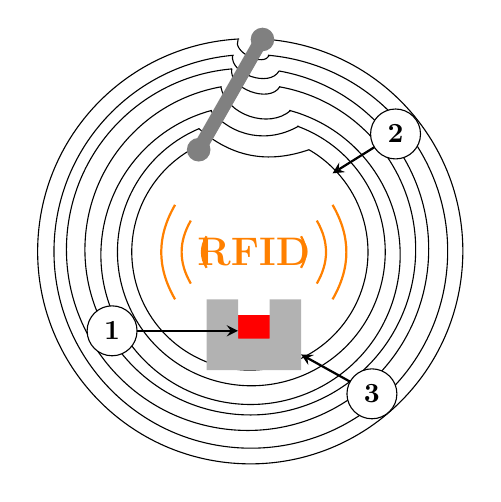
\begin{tikzpicture}
		
		% Spiral Antenna
		\draw (0.7,1.3)arc(60:-240:1.5);
		\draw (0.55,1.6)arc(70:-247:1.7);
		\draw (0.45,1.8)arc(75:-255	:1.9);
		\draw (0.32,2.1)arc(80:-260:2.1);
		\draw (0.32,2.3)arc(80:-265:2.3);
		\draw (0.18,2.5)arc(85:-265:2.5);
		\draw (0.19,2.7)arc(85:-267:2.7);
		
		\draw (-0.7,1.57)to [bend right](0.7,1.3);
		\draw(-0.55,1.8)to [bend right=40](0.57,1.6);
		\draw (-0.42,2.1)to [bend right=60](0.47,1.8);
		\draw (-0.28,2.33)to [bend right=80](0.33,2.1);
		\draw(-0.27,2.5)to [bend right=80](0.32,2.3);
		\draw(-0.20,2.7)to [bend right=90](0.20,2.50);
		
		% RFID Label
		\node[text=orange, font=\bfseries\Large] at (0,0) {RFID};
		\draw[orange, thick] (1,-0.6)   to [bend right](1,0.6);
		\draw[orange, thick] (0.8,-0.4) to [bend right](0.8,0.4); 
		\draw[orange, thick] (0.6,-0.2) to [bend right](0.6,0.2); 
		\draw[orange, thick] (-1,-0.6)  to [bend left](-1,0.6); 
		\draw[orange, thick] (-0.8,-0.4)to [bend left](-0.8,0.4); 
		\draw[orange, thick] (-0.6,-0.2)to [bend left](-0.6,0.2);  
		
		
		% RFID Chip
		\fill[red] (-0.2,-1.2) rectangle (0.2,-0.8);
		
		% Substrate
		\fill[gray!60] (-0.6,-1.5) -- (-0.6,-0.6) -- (-0.2,-0.6) -- (-0.2,-1.1)
		-- (0.2,-1.1) -- (0.2,-0.6) -- (0.6,-0.6) -- (0.6,-1.5) -- cycle;
		
		% Numbered circles with arrows
		\draw[-stealth, thick] (-1.8,-1) -- (-0.2,-1);
		\node[draw=black, fill=white, circle] at (-1.8,-1) {\textbf{1}};
		
		\draw[-stealth, thick] (1.8,1.5) -- (1.0,1.0);
		\node[draw=black, fill=white, circle] at (1.8,1.5) {\textbf{2}};
		
		\draw[-stealth, thick] (1.5,-1.8) -- (0.6,-1.3);
		\node[draw=black, fill=white, circle] at (1.5,-1.8) {\textbf{3}};
		\fill[gray] (0.11,2.7) circle(0.15);
		\fill[gray] (-0.7,1.3) circle(0.15);
		\draw[gray, line width=5pt] (-0.7,1.3) -- (0.1,2.7);
		
		
	\end{tikzpicture}
	%\includegraphics[width=1\linewidth]{../../../Manual/Images/Fotos-Hardware/RFID-Tag}
	\caption{Interner Aufbau eines passiven Transponders nach \cite{Conrad:2024a}}
	\label{fig:rfid-tag}
\end{figure}


























%
%
%\begin{figure}[H]
%	\centering
%	\begin{tikzpicture}[
%		block/.style={draw, thick, minimum width=3.2cm, minimum height=1.6cm, align=center},
%		arrow/.style={->, thick},
%		energy/.style={->, thick, red},
%		data/.style={->, thick, blue, dashed}
%		]
%		
%		% Microcontroller
%		\node[block, fill=blue!10] (mcu) {Mikrocontroller \\ (Master)};
%		
%		% RFID Reader
%		\node[block, right=4cm of mcu, fill=green!10] (reader) {RFID-Reader RC522 \\ (Slave)};
%		
%		% RFID Transponder
%		\node[block, right=4cm of reader, fill=orange!10] (tag) {RFID-Transponder};
%		
%		% Verbindung MCU <-> Reader
%		\draw[<->, thick] (mcu.east) -- (reader.west) node[midway, above] {\small SPI-Kommunikation};
%		
%		% Energiefluss Reader -> Tag
%		\draw[energy] (reader.east) ++(0,0.3) -- ++(3.5,0) node[midway, above, text=red] {\small Energie};
%		
%		% Datenfluss Tag -> Reader
%		\draw[data] (tag.west) ++(0,-0.3) -- ++(-3.5,0) node[midway, below, text=blue] {\small UID / Daten};
%		
%	\end{tikzpicture}
%	\caption{Vereinfachte Darstellung der Kommunikation zwischen Mikrocontroller (Master), RC522 (Slave) und RFID-Transponder}
%	\label{fig:rfid-kommunikation}
%\end{figure}
%




%%%%%%%%%% TIKZ-Kommunikation Mikrocontroller - RC522 - Transponder %%%%%%%%%%%%%%%%%%%%%

%
%
%\clearpage
%\begin{figure}[!ht]
%	\centering
%	\resizebox{1\textwidth}{!}{%
%		\begin{circuitikz}
%			\tikzstyle{every node}=[font=\LARGE]
%			\draw (2.5,11.5) to[short] (2.5,11.5);
%			\draw [ color={rgb,255:red,158; green,102; blue,5} , fill={rgb,255:red,238; green,191; blue,63}, dashed] (2.5,11.5) rectangle  (6.25,9);
%			\draw [ color={rgb,255:red,10; green,154; blue,174} , fill={rgb,255:red,4; green,163; blue,195}] (10,11.5) rectangle (15,9);
%			\draw [ fill={rgb,255:red,17; green,53; blue,197} ] (22.75,10.25) ellipse (2.25cm and 1.5cm);
%		\end{circuitikz}
%	}%
%	\label{fig:my_label}
%\end{figure}
%



%Das \ac{rc522} ist ein weit verbreitetes \ac{rfid}-Lesemodul, das auf dem \ac{mfrc522}-Chip von NXP Semiconductors basiert. 
%Es arbeitet im \ac{hf}-Bereich bei einer Frequenz von 13,56~MHz und unterstützt den Standard ISO/IEC~14443~A. 
%Mit diesem Modul können sowohl kontaktlose Karten als auch Transponder-Tags ausgelesen und beschrieben werden. 
%Einsatzgebiete sind unter anderem Zutrittskontrollsysteme, Authentifizierungsprozesse oder Prototypenentwicklungen \cite{nxpMFRC522,Handsontec:2023}.
%










%\subsection{Technische Spezifikationen}
%Die wichtigsten Eigenschaften des \ac{rc522}-Moduls sind in Tabelle~\ref{tab:rc522_specs} dargestellt.
%
%\begin{table}[H]
%	\centering
%	\caption{Technische Daten des \ac{rc522} nach \cite{Handsontec:2023}}
%	\label{tab:rc522_specs}
%	\begin{tabular}{ll}
%		\toprule
%		\textbf{Eigenschaft} & \textbf{Wert} \\
%		\midrule
%		Chip & \ac{mfrc522} \\
%		Betriebsspannung & 2,5–3,3~V \\
%		Betriebsstrom & 13–26~mA \\
%		Standby-Strom & 10–13~mA \\
%		Frequenz & 13,56~MHz (\ac{hf}) \\
%		Kommunikation & \ac{spi} (bis 10~Mbit/s), \ac{i2c} (bis 3,4~Mbit/s), \ac{uart} (bis 1228,8~kBd) \\
%		Unterstützte Standards & ISO/IEC~14443~A, MIFARE, NTAG \\
%		Reichweite & bis zu 50~mm (abhängig von Antenne/Tag) \\
%		\bottomrule
%	\end{tabular}
%\end{table}
%
%







%
%\subsection{Mifare RC522 RFID-Empf\"anger}
%Der Mifare RC522 RFID-Empf\"anger besteht, wie in Abbildung~\ref{fig:rfid-tag} zu sehen, aus einem integrierten Schaltkreis (IC) und einer Kupferspule, die als Antenne fungiert. Der Empf\"anger erzeugt, wie in Abbildung~\ref{fig:rfid-transpondererkennung} zu sehen, ein elektromagnetisches Feld, welches RFID-Tags in der N\"ahe aktiviert. Wenn ein Tag in das Feld gelangt, induziert die Antenne des Tags eine Spannung, die den Chip des Tags aktiviert. Dieser Chip sendet daraufhin eine eindeutige Identifikationsnummer (UID) an den RC522 zur\"uck.
%Der RC522 erfasst diese ID und kommuniziert sie \"uber die SPI-Schnittstelle (Serial Peripheral Interface) an den Arduino zur weiteren Verarbeitung. Der Empf\"anger ist darauf ausgelegt, zuverl\"assig in einem Bereich von 2,5cm bis 10cm zu arbeiten.
%
%    \begin{figure}
%        \centering
%        \includegraphics[width=1\linewidth]{../../../Manual/Images/Fotos-Hardware/RFID-Transpondererkennung}
%         \caption{RFID-Transpondererkennung\cite{Conrad:2024a}}
%         \label{fig:rfid-transpondererkennung}
%    \end{figure}







\subsection{Spezifikationen}

Die folgende Tabelle zeigt die technischen Spezifikationen des RFID-Moduls RC522 aus dem Datenblatt \cite{Handsontec:2023} auf einen Blick.

\begin{table}[H]
	\centering
	\caption{Technische Spezifikationen RC522-Modul \cite{Handsontec:2023,NXP:2016}}
	\label{tab:rc522_specs}
	\begin{tabular}{|l|p{9cm}|}
		\hline
		IC-Chip & MFRC522 von NXP \\
		\hline
		Betriebsspannung & \SI{2,5}{V} -- \SI{3,3}{V} (logikseitig \SI{3,3}{V}-kompatibel) \\
		\hline
		Frequenz & \SI{13,56}{MHz} (\ac{hf}-Band) \\
		\hline
		Stromaufnahme (aktiv) & \SI{13}{mA} -- \SI{26}{mA} \\
		\hline
		Stromaufnahme (Standby) & \SI{10}{mA} -- \SI{13}{mA} \\
		\hline
		Stromaufnahme (Sleep-Modus) & < \SI{8}{mA} \\
		\hline
		Kommunikationsschnittstellen & SPI, I\textsuperscript{2}C oder UART \\
		\hline
		Unterstützte Standards & ISO/IEC~14443~A (MIFARE Classic, Ultralight, NTAG) \\
		\hline
		Reichweite & typ. bis \SI{60}{mm} (abhängig von Antenne und Transponder) \\
		\hline
		Abmessungen Modul & ca. \SI{40}{mm} $\times$ \SI{50}{mm} \\
		\hline
		Betriebstemperatur & \SI{-25}{\degreeCelsius} bis \SI{+85}{\degreeCelsius} \\
		\hline
	\end{tabular}
\end{table}


Relevant ist hier die Kompatibilität zu 3,3~V-Logik, wodurch das Modul ohne zusätzliche Pegelwandler 
in Kombination mit Mikrocontrollern wie dem Arduino Nano 33 BLE Sense Lite betrieben werden kann.


\subsection{Aufbau des Moduls} 

Wie in Abbildung~\ref{fig:rc522_modul} zu sehen, umfasst das RC522-Modul neben dem zentralen \ac{mfrc522}-Chip weitere Bauteile, die für einen stabilen Betrieb erforderlich sind. 
Die Antenne ist als Leiterbahn in Spulenform direkt auf der Platine ausgeführt und wird durch zwei Induktivitäten (L1, L2) sowie elf Kondensatoren (C1--C11) unterstützt, die gemeinsam den Resonanzkreis für die Funkübertragung bei 13,56~MHz bilden. 
Ein Quarzoszillator liefert den Systemtakt für den Chip \cite{Handsontec:2023}. 
Fünf Widerstände (R1--R5) übernehmen Aufgaben wie Strombegrenzung und Signalführung. 
Zusätzlich ist eine Leuchtdiode (D1) integriert, die den Versorgungszustand anzeigt und somit eine optische Kontrolle ermöglicht. 
Der Anschluss an externe Systeme erfolgt über eine achtpolige Stiftleiste, die die Nutzung von \ac{spi}-, \ac{i2c}- oder \ac{uart}-Schnittstellen erlaubt.

\subsubsection{Pinbelegung}

Die achtpolige Stiftleiste, welche in Abbildung \ref{fig:rc522_modul} zu sehen ist, stellt die für den Betrieb benötigten Signale bereit. 
In der typischen SPI-Konfiguration ergibt sich die in Tabelle~\ref{tab:rc522_pinbelegung} dargestellte Zuordnung:

\begin{table}[H]
	\centering
	\caption{Pinbelegung des \ac{rc522} \cite{Handsontec:2023}}
	\label{tab:rc522_pinbelegung}
	\begin{tabular}{lll}
		\toprule
		\textbf{Pin} & \textbf{Bezeichnung} & \textbf{Funktion} \\
		\midrule
		1 & SS   & Slave Select \\
		2 & SCK  & SPI-Taktleitung \\
		3 & MOSI & Datenleitung Master $\rightarrow$ Slave \\
		4 & MISO & Datenleitung Slave $\rightarrow$ Master \\
		5 & IRQ  & Interrupt-Ausgang (optional) \\
		6 & GND  & Masse \\
		7 & RST  & Reset-Eingang \\
		8 & 3.3V & Spannungsversorgung \\
		\bottomrule
	\end{tabular}
\end{table}

Die Pins SS, SCK, MOSI und MISO bilden die SPI-Schnittstelle. 
GND und 3,3~V dienen der Spannungsversorgung, RST ermöglicht das Zurücksetzen des Moduls. 
Der IRQ-Pin wird in Standardanwendungen meist nicht benötigt, kann aber für spezielle Ereignissteuerungen genutzt werden.

\bigskip


    \begin{figure}
	\centering
	
\includegraphics[width=1\linewidth]{Sensor/RFIDRC522/RC522Modul.png}
	\caption{Bauteilübersicht des RC522-Moduls}
	\label{fig:rc522_modul}
	\end{figure}


\Mynote{Platzhalter für Tikz - mit hervorhebung durch Schablone und die Stiftleiste mit farblicher Kabelfarbe wie in der folgenden Tabelle}








\subsection{Anbindung an den Mikrocontroller}



Nach der Beschreibung der Spezifikationen und des Aufbaus des Moduls wird im Folgenden die konkrete Anbindung an den Arduino Nano 33 BLE Sense Lite erläutert. 


\bigskip

Für die Kommunikation zwischen dem Mikrocontroller und dem RFID-Modul RC522 wird die serielle \ac{spi}-Schnittstelle verwendet. 


Dabei ist zu beachten, dass der Pin \emph{SS} (Slave Select) für die Auswahl des Moduls genutzt wird. 
Die Bezeichnung SDA, die auf manchen Modulen anstelle von SS zu finden ist, bezieht sich ausschließlich auf die alternative I\textsuperscript{2}C-Schnittstelle und darf im SPI-Betrieb nicht verwendet werden.

Der Anschluss der Signale erfolgt über die achtpolige Stiftleiste des Moduls, wobei der IRQ-Pin nicht genutzt wird. 
IRQ dient als Interrupt-Ausgang, über den das Modul bestimmte Ereignisse an den Mikrocontroller melden kann, wird jedoch für grundlegende Lese- und Schreibvorgänge nicht benötigt. 

Die folgende Tabelle~\ref{tab:rc522_arduino} zeigt die Zuordnung der Pins des Moduls zum Arduino Nano 33 BLE Sense Lite sowie die verwendeten Kabelfarben, die zur einheitlichen Übersicht in der Verdrahtung beibehalten werden. 
Zu beachten ist außerdem, dass der Betrieb ausschließlich mit 3,3~V erfolgt, da der \ac{mfrc522}-Chip nicht 5~V-tolerant ist \cite{Handsontec:2023}.





\begin{table}[H]
	\centering
	\begin{tabular}{|c|c|c|c|}
		\hline
		\textbf{RC522-Pin} & \textbf{Nano 33 BLE} & \textbf{Funktion} & \textbf{Kabelfarbe} \\
		\hline
		\textcolor{red}{VCC} & 3.3V & Stromversorgung & \cellcolor{red!20}rot \\
		\hline
		\textcolor{black}{GND} & GND & Masse (Ground) & \cellcolor{black!10}schwarz \\
		\hline
		\textcolor{white!50!black}{SDA / SS} & D10 & Slave Select (Chip Select) & \cellcolor{gray!10}weiß \\
		\hline
		\textcolor{yellow!70!orange}{SCK} & D13 & SPI-Takt & \cellcolor{yellow!40}gelb \\
		\hline
		\textcolor{green!50!black}{MOSI} & D11 & Master Out → Slave In & \cellcolor{green!20}grün \\
		\hline
		\textcolor{blue}{MISO} & D12 & Master In ← Slave Out & \cellcolor{blue!20}blau \\
		\hline
		\textcolor{violet}{RST} & D9 & Reset & \cellcolor{violet!20}violett \\
		\hline
	\end{tabular}
	\caption{Anbindung des Moduls RC522  mit dem Arduino Nano 33 BLE Sense Lite}
	\label{tab:rc522_arduino}
\end{table}




 
















%%%%%%%%%%%%%%%%%%%%%%%%% TIKZ RC522   %%%%%%%%%%%%%%%%%%%%%%%%%%%%%%%%%%%%%%%%%%%%%%%%%%%%%%%%%%%%%%%%%%%%%%%%%
%%%%%%%%%%%%%%%%%%%%%%%%%%%%%%%%%%%%%%%%%%%%%%%%%%%%%%%%%%%%%%%%%%%%%%%%%%%%%%%%%%%%%%%%%%%%%%%%%%%%%%%%%%%%%%%%
%\begin{figure}
%	\centering
%	\begin{tikzpicture}[scale=1.2]
%		
%		% Vergrößerte Platine
%		\fill [blue!50!black](1,3) rectangle (7,11);
%		
%		% RFID Antennenringe (um 1.5 hoch verschoben)
%		\foreach \r in {0.6, 1.2, 1.8, 2.4} {
%			\draw[white] (4,7.5) circle (\r cm);
%		}
%		
%		% Dreiecke oben/unten (um 1.5 hoch verschoben)
%		\filldraw[fill=blue!50!black, draw=blue!50!black]
%		(4,7.5) -- (2,10.1) -- (6,10.1) -- cycle;
%		\filldraw[fill=blue!50!black, draw=blue!50!black]
%		(4,7.5) -- (2,4.9) -- (6,4.9) -- cycle;
%		
%		% RFID-Zentrum
%		\fill[white] (4,7.5) circle (0.25cm);
%		\node[white] at (4,5) {\textbf{MFRC522 Chip}};
%		
%		% Bohrlöcher
%		\foreach \x/\y in {1.5/3.5, 1.5/10.5, 6.5/3.5, 6.5/10.5} {
%			\fill [white] (\x,\y) circle (0.25cm);
%		}
%		
%		% Zentrierte 8 Pins in einer Reihe
%		% Gesamtlänge: 8 Pins * 0.6 + 7 Abstände * 0.2 = 6.8 cm
%		% Start bei x = 4 - 6.8/2 = 0.6 → x = 0.6
%
%\foreach \i/\name in {
%	0/VCC,
%	1/RST,
%	2/GND,
%	3/MISO,
%	4/MOSI,
%	5/SCK,
%	6/NSS,
%	7/IRQ
%} {
%	% Berechne die x-Koordinate des Mittelpunkts für den Bereich von 2.5 bis 5.5
%	\pgfmathsetmacro\x{2.5 + \i * (3/7)} % Abstand von 2.5 bis 5.5, gleichmäßig verteilt
%	\filldraw[fill=black!70] (\x - 0.2, 3.2) rectangle +(0.4, 0.4); % Rechtecke
%	\node[anchor=center, text=black, rotate=90] at (\x, 2.5) {\name}; % Text vertikal und zentriert
%}
%
%	\end{tikzpicture}
%
%	\caption{MFRC522 RFID Sensor nach \cite{AZDelivery2025}}
%	\label{fig:mfrc522}
%\end{figure}
%
%
%
%
%% -------- settings you can tweak --------
%\definecolor{pcb}{RGB}{23,76,130}       % Board blue
%\definecolor{silk}{RGB}{240,240,240}    % Silkscreen white
%\definecolor{copper}{RGB}{216,174,71}   % Gold pads
%\definecolor{shadow}{RGB}{10,35,70}     % Dark details
%\definecolor{soldermask}{RGB}{16,56,100}
%\newcommand\scaleBoard{0.9}             % overall scale
% ---------------------------------------
%%%%%%%%%%%%%%%%%%%%%%%%%%%%%%%%%%%%%%%%%%%%%%%%%%%%%%%%%%%%%%%%%%%%%%%%%%%%%%%%%%%%%%%%%%%%%%%%%%%%%%%%%%%%%%%%%%%%%%%%%%%
%%%%%%%%%%%%%%%%%%%%%%%%%%%%%%%%%%%%%%%%%%%%%%%%%%%%%%%%%%%%%%%%%%%%%%%%%%%%%%%%%%%%%%%%%%%%%%%%%%%%%%%%%%%%%%%%%%%%%%%%%%%%
%
%\begin{tikzpicture}[x=1cm,y=1cm,scale=.95,line cap=round,line join=round]
%	
%	% --- Board ---
%	\def\W{14.4}\def\H{9.0}\def\r{0.26}
%	\fill[pcb,rounded corners=\r cm] (0,0) rectangle (\W,\H);
%	
%	% --- Antenne (wie zuvor, gekürzt) ---
%	\def\ax{0.6}\def\ay{0.6}\def\aw{9.2}\def\ah{7.8}
%	\foreach \i in {0,...,8}{
%		\draw[silk,line width=0.6pt,rounded corners=0.35cm]
%		({\ax+0.20+0.38*\i},{\ay+0.20+0.38*\i})
%		rectangle ({\ax+\aw-0.20-0.38*\i},{\ay+\ah-0.20-0.38*\i});
%	}
%	
%	% --- 8-Pin Header (Fix: alle Rechnungen vorher auswerten) ---
%	\def\hx{13.15}
%	\def\hy{1.0}
%	\def\hpitch{0.6}
%	\def\pins{8}
%	
%	% Trägerrechteck: y-Top vorrechnen
%	\pgfmathsetmacro{\headertop}{\hy + (\pins-1)*\hpitch + 0.35}
%	\pgfmathsetmacro{\headerbot}{\hy - 0.35}
%	\fill[shadow,rounded corners=0.06cm]
%	(\hx-0.55,\headerbot) rectangle (\hx+0.55,\headertop);
%	
%	% Pins (oben 3.3V ... unten SDA)
%	\foreach \i/\name in {0/{3.3V},1/RST,2/GND,3/IRQ,4/MISO,5/MOSI,6/SCK,7/SDA}{
%		% y der Pinmitte (oben beginnend) vorrechnen:
%		\pgfmathsetmacro{\yy}{\hy + (\pins-1-\i)*\hpitch}
%		% Lötauge + schwarzer Kern
%		\fill[silk] (\hx-0.42,\yy) rectangle (\hx-0.12,\yy+0.28);
%		\fill[black] (\hx-0.40,\yy+0.02) rectangle (\hx-0.14,\yy+0.26);
%		% Label rechts
%		\node[anchor=west,inner sep=1pt,scale=0.8,text=silk]
%		at (\hx+0.65,\yy+0.14) {\name};
%	}
%	
%	% --- Rest (Dummy-Elemente, optional) ---
%	\fill[shadow,rounded corners=0.06cm] (10.5,3.2) rectangle (11.5,4.2);
%	\foreach \j in {0,...,5}{
%		\fill[copper,rounded corners=0.04cm]
%		({10.95+0.32*\j},{4.23}) rectangle ({11.2+0.32*\j},{5.15});
%	}
%	
%\end{tikzpicture}
%
%



%%%%%%%%%%%%%%%%%%%%%%%%%%%%% Pinbelegung  %%%%%%%%%%%%%%%%%%%%%%%%%%%%%%%%%%%%%%

%Mithilfe der Tabelle ann die Pinbelegung für den Nano33BLESense festgelegt werden.
%Die folgende Tabelle~\ref{fig:PinbelegungSensor} zeigt eine M\"ogliche Pinbelegung zwischen dem RFID-Modul und dem Arduino. Daraus abgeleitet wurde die Pinbelegung zwischen dem RFID-Modul und dem Nano33BLESense. Das RFID-Modul eignet sich für die Verwendung mit anderen Mikrocontrollern. Die Pins müssen ggf. angepasst werden. F\"ur den Simple Code (Listing:~\ref{lst:simplecode}) und Simple Application (Listing:~\ref{lst:simpleapplication}) sollte die in der Tabelle gezeigte Pinbelegung eingehalten werden.
%Der IQR-Pin des RFID-Moduls wird in diesem Fall nicht verwendet. Bei diesem Projekt wird die Verwendung nicht benötigt und kann daher weggelassen werden.

%%Tabelle Pinbelegung Nano33BLESense
%\begin{table}
%	\centering
%	\caption{Pinbelegung RC522 mit Arduino Nano BLE Sense nach \cite{AZDelivery2025}\label{fig:PinbelegungSensor}}
%	\begin{tabular}{|l|l|l|l|}
%		\hline
%		\textbf{RFID Sensor Pin} & \textbf{Grove Shield Pin} & \textbf{Arduino Pin} & \textbf{Funktion} \\ \hline
%		SDA  & 5 & D8   & SS / Slave Select 		\\ \hline
%		SCK  & 12& D3   & SCK / Serial Clock 		\\ \hline
%		MISO & 9 & D4   & MISO / Master In Slave Out \\ \hline
%		MOSI & 11& D5   & MOSI / Master Out Slave In \\ \hline
%		RST  & 8 & D9   & Reset 						\\ \hline
%		GND  & 2 & GND  & Masse / Ground 			\\ \hline
%		3.3V & 1 &3.3V & Versorgungsspannung			\\ \hline
%	\end{tabular}
%\end{table}

%Das RFID-Modul wird nicht direkt an den Nano33BLESense angeschlossen. Zur Verbindung der Komponenten wird das Shield aus dem TinyML-Kit verwendet. Folgendes Bild \ref{fig:pins_shield} zeigt die Pinbelegung an der KameraSteckverbindung des  machinelearningShields:
%
%\begin{figure}
%	\centering
%	\caption{Pins des Shields nach  \cite{ArduinoShield:2021} und \ref{TinyMachineLearningShieldPins}}\label{fig:pins_shield}
%	\begin{tikzpicture}[scale=0.7]
%		
%		% Rechteck
%		\draw[thick] (5, 0) rectangle (7, 11);
%		
%		% Linien mit Beschriftung und Innenbeschriftung
%		\foreach \y/\leftlabel/\rightlabel/\leftdesc/\rightdesc in {
%			1/19/20//,
%			2/17/18//,
%			3/15/16//,
%			4/13/14//,
%			5/11/12/ MOSI/SCK,
%			6/9/10/MISO/,
%			7/7/8//Reset,
%			8/5/6/SDA/,
%			9/3/4//,
%			10/1/2/ /
%		} {
%			% Sonderfall: 3 V (Linie 10)
%			\ifnum\y=10
%			\draw[thick] (2.5,\y) -- (5,\y); % linke Linie gekürzt
%			\node[anchor=center] at (6,\y) {\leftlabel\quad\quad\rightlabel}; % Rechteck-Beschriftung
%			\node[anchor=west] at (2.5,\y) {\leftdesc}; % Beschreibung links
%			\node[anchor=east] at (9.5,\y) {\rightdesc}; % Beschreibung rechts
%			\draw[thick] (2.5,9.5) -- (2.5,10.5); % senkrechte 3V Linie
%			\node[left] at (2.5, 10) {3.3~V};
%			\draw[thick] (9.5,9.5) -- (9.5,10.5); % GND Linie
%			\draw[thick] (9.6,9.6) -- (9.6,10.4);
%			\draw[thick] (9.7,9.7) -- (9.7,10.3);
%			\draw[thick] (9.8,9.8) -- (9.8,10.2);
%			\node[right] at (9.8, 10) {GND};
%			\draw[thick] (7,\y) -- (9.5,\y); % rechte Linie ganz
%			% Sonderfall: GND (Linie 9)
%			\else\ifnum\y=9
%			% Sonderfall GND hier behandeln (falls benötigt)
%			\draw[thick] (0,\y) -- (5,\y); % linke Linie
%			\draw[thick] (7,\y) -- (12,\y); % rechte Linie
%			\node[anchor=center] at (6,\y) {\leftlabel\quad\quad\rightlabel}; % Zahlen im Rechteck
%			\node[anchor=west] at (-1,\y) {\leftdesc}; % Beschreibung links
%			\node[anchor=east] at (13,\y) {\rightdesc}; % Beschreibung rechts
%			% Alle anderen Pins
%			\else
%			\draw[thick] (0,\y) -- (5,\y); % linke Linie
%			\draw[thick] (7,\y) -- (12,\y); % rechte Linie
%			% Zahlen im Rechteck (weiter auseinander)
%			\node[anchor=center] at (6,\y) {\leftlabel\quad\quad\rightlabel}; % Zahlen im Rechteck
%			\node[anchor=west] at (-2,\y) {\leftdesc}; % Beschreibung links
%			\node[anchor=east] at (14,\y) {\rightdesc}; % Beschreibung rechts
%			\fi\fi
%		}
%	\end{tikzpicture}
%\end{figure}















%
%\section{Bibliothek \PYTHON{Easy MFRC522}}
%
%Damit der Arduino Nano 33 BLE Sense Lite mit dem Modul RC522 arbeiten kann, 
%werden passende Softwarebibliotheken benötigt. 
%Bibliotheken enthalten bereits vorbereitete Befehle und Funktionen, 
%die den Zugriff auf die Hardware deutlich vereinfachen. 
%Anstatt jede einzelne Anweisung selbst zu programmieren, 
%können durch Bibliotheken vorhandene Routinen genutzt werden, 
%um die Kommunikation zwischen dem Mikrocontroller und dem Modul sicher und zuverlässig zu gestalten. 
%
%Ohne solche Bibliotheken müsste jede Funktion des Moduls manuell über Register programmiert werden, 
%was sehr aufwendig und fehleranfällig wäre. 
%Die Verwendung von Bibliotheken sorgt daher für eine übersichtlichere Programmstruktur 
%und eine schnellere Entwicklung.
%













\section{Bibliotheken}



Damit der Arduino Nano 33 BLE Sense Lite mit dem Modul RC522 zusammenarbeiten kann, 
müssen passende Softwarebibliotheken eingebunden werden. 
Diese Bibliotheken enthalten bereits vorbereitete Funktionen, 
um die Kommunikation zwischen dem Mikrocontroller und dem Modul über die SPI-Schnittstelle zu ermöglichen. 
Dadurch entfällt die Notwendigkeit, einzelne Register des Moduls direkt anzusprechen.


\subsection{Bibliothek \PYTHON{Easy MFRC522}}

Für die Ansteuerung des Moduls RC522 wird die Bibliothek \PYTHON{Easy MFRC522} 
von Pablo Sampaio \cite{Sampaio:2025} verwendet. 
Sie basiert auf der ursprünglichen Bibliothek \PYTHON{MFRC522} von Miguel Balboa \cite{Balboa:2025}, 
die als Standardbibliothek für das Modul RC522 in der Arduino-Umgebung gilt. 

Die Bibliothek \PYTHON{Easy MFRC522} vereinfacht viele typische Vorgänge, 
indem sie wiederkehrende Abläufe – wie das Aktivieren des Moduls, 
das Lesen oder Schreiben von Datenblöcken sowie das Beenden einer Übertragung – automatisch ausführt. 
Dadurch wird der Programmcode deutlich kürzer und übersichtlicher, 
und die Entwicklung von Anwendungen mit dem Modul RC522 wird erleichtert. 

Unterstützt werden Transponder der Mifare-Classic-Familie (Mini, 1K, 4K). 
Für die Authentifizierung wird ausschließlich der Schlüsseltyp Key A verwendet, 
wobei alle beteiligten Speicherblöcke denselben Schlüssel nutzen müssen \cite{Sampaio:2025}.


\begin{tcolorbox}[colback=gray!10, colframe=gray!60, title={Hinweis zur Bibliothek \PYTHON{Easy MFRC522}}]
	
	Die Bibliothek \PYTHON{Easy MFRC522} von Pablo Sampaio ist eine vereinfachte Weiterentwicklung 
	der Standardbibliothek \PYTHON{MFRC522} von Miguel Balboa. 
	Ihr Hauptzweck besteht darin, den Zugriff auf das Modul RC522 zu vereinfachen 
	und das Auslesen der \ac{uid} von \ac{rfid}-Transpondern zu ermöglichen, 
	ohne dass komplexe Protokollschritte manuell programmiert werden müssen. 
	
	Für die Authentifizierung wird ausschließlich der Schlüsseltyp \textbf{Key A} 
	mit dem Standardwert \texttt{FF FF FF FF FF FF} verwendet. 
	Dadurch ist die Bibliothek besonders geeignet für Anwendungen, 
	bei denen die eindeutige Identifikation eines Transponders (z.\,B. in einer Zutrittskontrolle) 
	ausreichend ist. 
	
	Das Schreiben oder Lesen eigener Daten auf den Speicherblöcken eines Transponders 
	ist grundsätzlich möglich, jedoch nur solange der Standard-Key A verwendet wird. 
	Eine Authentifizierung über \textbf{Key B} oder die Nutzung benutzerdefinierter Schlüssel 
	wird von dieser Bibliothek nicht unterstützt \cite{Sampaio:2025}. 
	Für erweiterte Funktionen wie sektorweises Schreiben, individuelle Schlüssel oder 
	Zugriffskontrollen sollte daher die Bibliothek \PYTHON{MFRC522} von Miguel Balboa verwendet werden.
\end{tcolorbox}



\subsection{Bibliothek \FILE{SPI.h}}

Die Bibliothek \FILE{SPI.h} ist eine zentrale Systembibliothek der Arduino-Entwicklungsumgebung 
und ermöglicht die Kommunikation über die Schnittstelle SPI. 
Das Protokoll SPI ist ein schnelles, synchrones Datenübertragungsverfahren, 
das speziell für den Austausch zwischen einem Mikrocontroller und mehreren Peripheriegeräten entwickelt wurde. 

Mit Hilfe der Bibliothek können Daten seriell, also bitweise, übertragen werden. 
Die Kommunikation erfolgt dabei im Takt einer gemeinsamen Clock-Leitung SCK 
und nutzt vier Hauptsignalleitungen:

\begin{itemize}
	\item \textbf{MISO} (Master In Slave Out): Überträgt Daten vom Peripheriegerät zum Mikrocontroller,
	\item \textbf{MOSI} (Master Out Slave In): Überträgt Daten vom Mikrocontroller zum Peripheriegerät,
	\item \textbf{SCK} (Serial Clock): Gibt den Takt für die Datenübertragung vor,
	\item \textbf{SS} (Slave Select): Aktiviert das jeweils ausgewählte Peripheriegerät.
\end{itemize}

Die Bibliothek \FILE{SPI.h} stellt Funktionen bereit, 
mit denen sich die Schnittstelle initialisieren und Daten zuverlässig übertragen lassen. 
Beispiele dafür sind \PYTHON{SPI.begin()} zur Aktivierung der Schnittstelle, 
\PYTHON{SPI.transfer()} zum Senden und Empfangen einzelner Bytes 
sowie \PYTHON{SPI.endTransaction()} zum Beenden einer Übertragung. 

Durch die Verwendung dieser Bibliothek entfällt die manuelle Programmierung der Signalleitungen. 
Sie gewährleistet eine stabile Kommunikation und ermöglicht den gleichzeitigen Betrieb mehrerer SPI-Geräte, 
da jedes Gerät über eine eigene Slave-Select-Leitung individuell angesprochen werden kann.



\newpage





 
 \subsection{Installation der Bibliothek \PYTHON{Easy MFRC522}}\label{Libraryinstall}
 
 Die beschriebenen Bibliotheken bilden die Grundlage für die Kommunikation und Datenverarbeitung. 
 Dabei ist zu beachten, dass die Bibliothek \FILE{SPI.h} als Bestandteil der Arduino-Entwicklungsumgebung 
 bereits vorinstalliert ist und daher nicht manuell hinzugefügt werden muss. 
 Im folgenden Abschnitt wird die Installation der externen Bibliothek \PYTHON{Easy MFRC522} erläutert.
 
 
 \subsubsection{Installationsanweisung}
 
 Die Installation der Bibliothek \PYTHON{Easy MFRC522} erfolgt über die integrierte Bibliotheksverwaltung der Entwicklungsumgebung Arduino IDE. 
 Nach dem Start der Arduino IDE wird die Bibliotheksverwaltung über das entsprechende Symbol in der Symbolleiste (\textbf{1}) geöffnet, 
 wie in Abbildung~\ref{fig:library-open} dargestellt.
 
 \begin{figure}
 	\centering
 	
\includegraphics[width=1\linewidth]{Sensor/RFIDRC522/Library/OeffnenLibrary.png}
 	\caption{Öffnen der Bibliotheksverwaltung [eigene Darstellung]}
 	\label{fig:library-open}
 \end{figure}
 
 Im Suchfeld (\textbf{2}) wird anschließend der Name der Bibliothek \PYTHON{Easy MFRC522} eingegeben 
 (siehe Abbildung~\ref{fig:Libraryinstallation}). 
 Nach kurzer Ladezeit erscheint die entsprechende Bibliothek in der Ergebnisliste. 
 Die gewünschte Version (\textbf{3}) kann aus dem Auswahlmenü gewählt und über die Schaltfläche 
 \textbf{Installieren} hinzugefügt werden.
 
 \begin{figure}
 	\centering
 	
\includegraphics[width=1\linewidth]{Sensor/RFIDRC522/Library/Installation.png}
 	\caption{Auswahl und Installation der Bibliothek [eigene Darstellung]}
 	\label{fig:Libraryinstallation}
 \end{figure}
 
 Während der Installation öffnet sich ein Dialogfenster, 
 in dem mögliche Abhängigkeiten anderer Bibliotheken angezeigt werden (Abbildung~\ref{fig:LibraryAlleInstallieren}). 
 Mit einem Klick auf \textbf{Alle installieren} (\textbf{4}) werden diese automatisch ergänzt.
 
 \begin{figure}
 	\centering
 	
\includegraphics[width=1\linewidth]{Sensor/RFIDRC522/Library/AlleInstallieren.png}
 	\caption{Installationsdialog mit zusätzlichen Abhängigkeiten [eigene Darstellung]}
 	\label{fig:LibraryAlleInstallieren}
 \end{figure}
 
 Nach Abschluss des Installationsvorgangs wird der Status \enquote{Installiert} (\textbf{5}) angezeigt, 
 wie in Abbildung~\ref{fig:LibraryInstallationabgeschlossen} gezeigt. 
 Über die Schaltfläche \textbf{More info} (\textbf{6}) lassen sich zusätzliche Informationen 
 zur Bibliothek, wie Versionshinweise oder Quellverweise, einsehen.
 
 \begin{figure}
 	\centering
 	
\includegraphics[width=1\linewidth]{Sensor/RFIDRC522/Library/Installationabgeschlossen.png}
 	\caption{Abgeschlossene Installation der Bibliothek [eigene Darstellung]}
 	\label{fig:LibraryInstallationabgeschlossen}
 \end{figure}
 
 Nach der erfolgreichen Installation steht die Bibliothek \PYTHON{Easy MFRC522} 
 in der Arduino IDE zur Verfügung und kann durch den Befehl 
 \PYTHON{\#include <EasyMFRC522.h>} in den Quellcode eingebunden werden.
 


\section{Einfacher Code}

In diesem Beispiel wird die grundlegende Funktion des RFID-Moduls RC522 demonstriert. 
Wird ein Transponder auf das in Abbildung~\ref{fig:mfrc522} dargestellte Modul gelegt, 
so wird dessen eindeutige Kennung (UID) im seriellen Monitor der Arduino-IDE ausgegeben. 
Der dargestellte Quellcode \ref{lst:simplecodeuid} dient als erster Verbindungstest, 
um die Kommunikation zwischen dem Arduino Nano 33 BLE Sense Lite und dem RFID-Modul RC522 zu überprüfen 
und die grundlegende Funktionsfähigkeit der verwendeten Hardware sicherzustellen.

Das RFID-Modul RC522 wird gemäß dem im Anhang dargestellten Schaltplan (vgl. Abbildung~XY) 
an den Arduino Nano 33 BLE Sense Lite angeschlossen. 
Der Arduino Nano 33 BLE Sense Lite wird über ein Micro-USB-Kabel mit dem Computer verbunden, 
wodurch sowohl die Spannungsversorgung als auch die serielle Datenübertragung zur Arduino IDE erfolgt.

Über das Menü \menu{Tools > Serial Monitor} wird der serielle Monitor gestartet, 
und der Code wird auf den Mikrocontroller hochgeladen. 
Wird der serielle Monitor erst nach dem Upload geöffnet, 
erscheinen keine Ausgaben, da die Startsequenz bereits abgeschlossen ist. 
Nach dem erfolgreichen Programmstart erscheinen im Monitor die Meldungen 
\enquote{Hello World} und \enquote{Arduino RFID: Place tags one after another...}. 
Sobald diese angezeigt werden, können die Transponder nacheinander 
in einem Abstand von etwa \SI{5}{\centi\metre} an das RFID-Modul RC522 gehalten werden, 
wie im Datenblatt des Moduls beschrieben \cite{Handsontec:2023}. 
Die jeweilige UID des Transponders wird daraufhin im seriellen Monitor angezeigt 
(siehe Abbildung~\ref{fig:SimpleCodeUIDErkennung}).

\begin{code}
	\caption{Einfacher Code zum Auslesen der UID eines Transponders}
	\label{lst:simplecodeuid}
	\ArduinoExternal{}
	{../../Code/Nano33BLESense/SensorRFIDRC522/SimpleCodeUID/SimpleCodeUID.ino}
\end{code}

Für die Implementierung werden die Arduino-Standardbibliothek \FILE{SPI.h} 
zur Kommunikation über den SPI-Bus sowie die Bibliothek \FILE{MFRC522.h} 
zur Steuerung des RFID-Moduls verwendet. 
Zu Beginn erfolgt die Initialisierung der seriellen Schnittstelle über \PYTHON{Serial.begin()}, 
des SPI-Busses mit \PYTHON{SPI.begin()} und des RFID-Moduls über \PYTHON{rfid.PCD\_Init()}. 
Anschließend gibt das Programm eine kurze Startmeldung \enquote{Hello World} im seriellen Monitor aus. 

In der Hauptschleife \PYTHON{loop()} prüft das Programm fortlaufend, 
ob sich ein neuer Transponder in Reichweite befindet. 
Wird ein Transponder erkannt, 
so wird dessen UID ausgelesen und byteweise im Hexadezimalformat im seriellen Monitor ausgegeben 
(siehe Abbildung~\ref{fig:SimpleCodeUIDErkennung}). 
Nach dem Auslesen wird die Kommunikation mit dem Transponder beendet, 
und durch eine Verzögerung von 500~ms wird eine Mehrfacherkennung desselben Transponders verhindert.

\begin{figure}
	\centering
	
\includegraphics[width=1\linewidth]{Sensor/RFIDRC522/SimpleCode/SerialMonitorUIDOutcome}
	\caption{Ausgabe der UID im seriellen Monitor [eigene Darstellung]}
	\label{fig:SimpleCodeUIDErkennung}
\end{figure}




\newpage




\subsection{Funktionen zur Verwendung des RFID-Moduls RC522}

Im folgenden Abschnitt werden die im Beispielcode genutzten Funktionen beschrieben. 
Diese lassen sich zwei Bibliotheken zuordnen: \FILE{SPI.h} und \PYTHON{MFRC522.h}. 
Die Bibliothek \FILE{SPI.h} stellt die Verbindung zwischen dem Arduino und dem RFID-Modul RC522 her, 
während die Bibliothek \FILE{MFRC522.h} die Kommunikation und Steuerung des Moduls übernimmt. 
Zur besseren Übersicht sind die Funktionen nach diesen beiden Bibliotheken aufgeteilt.


\subsubsection*{1. Funktionen der Bibliothek \FILE{SPI.h}}

\begin{itemize}
	\item \PYTHON{SPI.begin()} – Initialisiert den SPI-Bus und aktiviert die serielle Kommunikation 
	zwischen dem Mikrocontroller und dem RFID-Modul RC522. 
	Diese Funktion muss zu Beginn des Programms aufgerufen werden, 
	damit die Datenübertragung über die SPI-Leitungen MISO, MOSI, SCK, SS funktioniert.
\end{itemize}

\subsubsection*{2. Funktionen der Bibliothek \FILE{MFRC522.h}}

\begin{itemize}
	\item \PYTHON{rfid.PCD\_Init()} – Initialisiert den RFID-Reader und stellt die Verbindung zum Modul RC522 her.
	\item \PYTHON{rfid.PICC\_IsNewCardPresent()} – Prüft, ob sich ein neuer Transponder im Lesebereich befindet.
	\item \PYTHON{rfid.PICC\_ReadCardSerial()} – Liest die eindeutige UID des erkannten Transponders.
	\item \PYTHON{rfid.uid.uidByte[]} – Bietet Zugriff auf die einzelnen Bytes der ausgelesenen UID.
	\item \PYTHON{rfid.PICC\_HaltA()} – Beendet die Kommunikation mit dem aktuell erkannten Transponder.
	\item \PYTHON{rfid.PCD\_StopCrypto1()} – Stoppt die zwischen Reader und Transponder aufgebaute Verschlüsselung.
\end{itemize}

\subsubsection*{3. Ergänzende Funktionen}

\begin{itemize}
	\item \PYTHON{Serial.begin(9600)} – Startet die serielle Schnittstelle, 
	um Statusmeldungen und ausgelesene Daten im seriellen Monitor anzuzeigen.
	\item \PYTHON{delay(500)} – Fügt eine kurze Pause von 500~ms ein, 
	um Mehrfacherkennungen desselben Transponders zu vermeiden.
\end{itemize}

Der erfolgreiche Test mit der Ausgabe im seriellen Monitor zeigt, 
dass die Kommunikation über den SPI-Bus ordnungsgemäß funktioniert 
und bestätigt den erfolgreichen Datenaustausch mit dem RFID-Modul RC522.

 


%%%%%%%% SPI-BUS %%%%%%%%%%%%%%%%%%%%%%%%%%%

%Beim SPI-Bus (Serial Peripheral Interface):
%
%Der Arduino (Master) steuert den Verkehr → er gibt den Takt (Clock) vor.
%
%Angeschlossene Module (Slaves, z. B. RC522 oder ein Display) hören zu oder antworten, wenn sie vom Master ausgewählt werden.
%
%Damit nicht alle gleichzeitig sprechen, hat jedes Gerät eine eigene SS-Leitung (Slave Select).
%
% Deshalb „Bus“: weil mehrere Geräte über die gleichen Leitungen verbunden werden können, aber immer nur eines aktiv mit dem Master spricht.

%%%%%%%%%%%%%%%%%%%%%%%%%%%%%%%%%%%%%%%%%%%%%%%%%%%%%%%%%%%%%%%%%%%%%%%%%%%%%%%%%%%%%%%%%%%%%%%%%%%%%%%%%%%





\newpage





\section{Einfache Anwendung}

\subsection{Autorisierung zugelassener Transponder}

Die Anwendung bildet den Ablauf einer RFID-basierten Zugangskontrolle ab. 
Sie überprüft, ob ein vorgehaltener Transponder in der Liste der zugelassenen Identifikatoren enthalten ist 
und gibt das Ergebnis über die integrierte LED des Arduino Nano 33 BLE Sense Lite sowie über den seriellen Monitor aus. 





\begin{code}
	\caption{Einfache Anwendung einer RFID-basierten Zugangskontrolle}
	\label{lst:simpleapplication}
	\ArduinoExternal{
	}{../../Code/Nano33BLESense/SensorRFIDRC522/SampleRFIDAccessControl/SampleRFIDAccessControl.ino}
\end{code}







\subsection{Beschreibung}

Das in Listing~\ref{lst:simpleapplication} dargestellte Programm nutzt das RFID-Modul RC522, 
um Transponder zu erfassen und deren eindeutige Identifikationsnummer, also die UID (Access Number), über die serielle Schnittstelle auszugeben. 
Wird ein Transponder erkannt, wird dessen Identifikationsnummer (UID) über das Modul \PYTHON{ModulMFRC522} ausgelesen 
und durch das Modul \PYTHON{AccessControl} überprüft. 
Je nach Ergebnis erfolgt eine optische Rückmeldung über die LED. 
Bleibt die Erkennung aus, wird keine Ausgabe erzeugt und die LED bleibt deaktiviert.

Die im seriellen Monitor angezeigte Ausgabe enthält jeweils die gelesene Access Number sowie den aktuellen Zugriffsstatus. 
Ein erfolgreicher Abgleich mit der hinterlegten Liste autorisierter Kennungen führt zur Ausgabe \enquote{Status=granted}, 
während bei nicht zugelassenen Transpondern \enquote{Status=denied} erscheint. 
Diese textbasierte Rückmeldung ermöglicht die Überprüfung der Programmlogik und zeigt gleichzeitig den korrekten Ablauf 
der Kommunikation zwischen dem Mikrocontroller und dem RFID-Modul. 
Eine beispielhafte Ausgabe ist in Abbildung~\ref{fig:SerialMonitorOutput} dargestellt.



\begin{figure}
	\centering
	
\includegraphics[width=1\linewidth]{Sensor/RFIDRC522/Sample/SerialMonitorOutcomeSample}
	\caption{Ausgabe im seriellen Monitor während der Authorisierungsanwendung}
	\label{fig:SerialMonitorOutput}
\end{figure}




\subsection{Code Aufbau}
Die zentrale Ablaufsteuerung erfolgt in der Datei \FILE{main.ino}, 
die die Initialisierung der Module übernimmt und den Programmfluss in der Hauptschleife \PYTHON{loop()} steuert. 
Verwendet werden die Module \PYTHON{AccessControl}, \PYTHON{ModulMFRC522} und \PYTHON{LEDBuiltin}. 
Die LED-Funktionalität entstammt den bereitgestellten Unterlagen und befindet sich im Pfad:  
\menu{Nano33BLESense > Code > Nano33BLESense > LEDs}. 

Die einzelnen Module sind jeweils in eine Header-Datei (\FILE{.h}) und eine Implementierungsdatei (\FILE{.cpp}) unterteilt. 
Diese Trennung dient der besseren Strukturierung und Wiederverwendbarkeit des Codes. 
In den Header-Dateien werden die Funktionsdeklarationen definiert, die anderen Programmteilen den Zugriff auf die jeweiligen Module ermöglichen. 
Die eigentliche Implementierung der Funktionen erfolgt in den zugehörigen \FILE{.cpp}-Dateien. 
Durch diese Aufteilung kann die Programmlogik klar gegliedert, Abhängigkeiten reduziert und der Quellcode übersichtlicher gestaltet werden.

Zu Beginn der Programmausführung werden die serielle Kommunikation, die interne LED und der RFID-Reader über die \ac{spi}-Schnittstelle initialisiert. 
Der Programmablauf folgt einer festen Reihenfolge:
\begin{enumerate}
	\item Erkennen eines Transponders.
	\item Auslesen der UID über \PYTHON{ModulMFRC522}.
	\item Prüfung der UID über \PYTHON{AccessControl}.
	\item Rückmeldung des Ergebnisses über die LED und den seriellen Monitor.
\end{enumerate}

Diese Struktur setzt das modulare Softwarekonzept konsequent um und bildet den vollständigen Ablauf einer Zugangskontrolle 
von der Erfassung des Transponders bis zur Ausgabe des Ergebnisses ab.




%\begin{code}
%	\caption{ModulMFRC522.h}
%	\label{lst:modulmfrc522.h}
%	\ArduinoExternal{
%	}{../../Code/Nano33BLESense/RC522RFID/SampleRFIDAccessControl/ModulMFRC522.h}
%\end{code}
%
%\begin{code}
%	\caption{ModulMFRC522.cpp}
%	\label{lst:modulmfrc522.cpp}
%	\ArduinoExternal{
%	}{../../Code/Nano33BLESense/RC522RFID/SampleRFIDAccessControl/ModulMFRC522.cpp}
%\end{code}
%
%\begin{code}
%	\caption{AccessControl.h}
%	\label{lst:acces.h}
%	\ArduinoExternal{
%	}{../../Code/Nano33BLESense/RC522RFID/SampleRFIDAccessControl/AccessControl.h}
%\end{code}
%
%\begin{code}
%	\caption{AccessControl.cpp}
%	\label{lst:access.cpp}
%	\ArduinoExternal{
%	}{../../Code/Nano33BLESense/RC522RFID/SampleRFIDAccessControl/AccessControl.cpp}
%\end{code}

%%%%%%%%%%%%%%%%%%%%%%%%%%%%%%%%%%%%%%%%%%%%%%%%%%%%%

%
%\section{Erste Tests}
%Das Ziel ist es herauszufinden, ob der RFID-Sensor richtig angeschlossen ist und funktioniert. Wichtig ist dabei auch das Feedback der LED des RFID-Sensors. Diese sollte leuchten, wenn der RFID-Sensor mit GND und 3.3~V verbunden ist. 
%Falls der Sensor den RFID-Tag nicht erkennt, sollte ein anderer RFID-Tag verwendet werden, um diesen als Fehlerquelle auszuschließen.
%\begin{itemize}
%	\item \textbf{Test:} Karte erkannt?
%	\item \textbf{Vorgehen:} Eine beliebige RFID-Karte oder ein Tag wird in die N\"ahe des Lesers gehalten.
%	\item \textbf{Erwartung:} Die UID der Karte wird korrekt und vollst\"andig im Serial Monitor ausgegeben.
%	\item \textbf{Hinweis:} Nach erfolgreicher Erkennung folgt eine Pause von einer Sekunde zur besseren Lesbarkeit.
%\end{itemize}


%
%\subsection{Test der Funktionen}
%
%\begin{itemize}
%	\item \PYTHON{PCD\_Init()} – \textbf{Test:} Initialisiert das MFRC522-Modul korrekt?\\
%	\PYTHON{Erwartung:} Modul reagiert nach dem Start zuverl\"assig auf RFID-Tags.\\
%	\textbf{Verwendete Funktion:} Wie in Listing~\ref{lst:simplecode} gezeigt, wird \PYTHON{PCD\_Init()} verwendet, um das MFRC522-Modul zu initialisieren.
%
%	\item \PYTHON{PICC\_IsNewCardPresent()} – \textbf{Test:} Erkennt das System eine neue Karte?\\
%	\textbf{Erwartung:} R\"uckgabewert ist \PYTHON{true}, wenn ein neuer Tag im Lesebereich erkannt wird.\\
%	\textbf{Verwendete Funktion:} Wie in Listing~\ref{lst:simpleapplication} gezeigt, wird \PYTHON{PICC\_IsNewCardPresent()} verwendet, um festzustellen, ob eine neue Karte verf\"ugbar ist.
%
%	\item \PYTHON{PICC\_ReadCardSerial()} – \textbf{Test:} Wird die UID korrekt gelesen?\\
%	\textbf{Erwartung:} Die UID wird vollst\"andig ausgelesen und korrekt angezeigt.\\
%	\textbf{Verwendete Funktion:} Wie in Listing~\ref{lst:simpleapplication} gezeigt, wird \PYTHON{PICC\_ReadCardSerial()} genutzt, um die UID der Karte zu lesen.
%
%	\item \PYTHON{unlockDoor()} – \textbf{Test:} \"Offnet und schliesst das Schloss wie erwartet?\\
%	\textbf{Erwartung:} \PYTHON{LOCK\_PIN} wird f\"ur eine definierte Zeit aktiviert (hier: 3000 ms).\\
%	\textbf{Verwendete Funktion:} Wie in Listing~\ref{lst:simpleapplication} gezeigt, wird \PYTHON{unlockDoor()} verwendet, um das T\"ur-Schloss zu steuern.
%
%	\item \PYTHON{MIFARE\_Write()} – \textbf{(optional)} \textbf{Test:} K\"onnen Daten erfolgreich auf eine Karte geschrieben und anschliessend gelesen werden?\\
%	\textbf{Erwartung:} Daten bleiben auf dem Tag gespeichert und sind korrekt lesbar.\\
%	\textbf{Verwendete Funktion:} Wie in Listing~\ref{lst:simpleapplication} gezeigt, k\"onnte \PYTHON{MIFARE\_Write()} verwendet werden, um Daten auf eine RFID-Karte zu schreiben (zus\"atzlicher Code erforderlich).
%\end{itemize}

\section{Weiterführende Literatur}

%Für ein vertieftes Verständnis des RFID-Moduls MFRC522 sowie seiner praktischen Anwendung empfiehlt sich die Beschäftigung mit weiterführender Literatur. Im Folgenden sind Quellen aufgeführt, die weiterführende Informationen bieten.
%
%\subsection{Offizielle NXP Dokumentation zum MFRC522}
%
%Die Anlaufstelle für technische Details zum MFRC522 ist die offizielle Dokumentation des Herstellers NXP Semiconductors. Das Datenblatt enthält Informationen über die elektrischen Eigenschaften, Kommunikationsschnittstellen sowie das Protokollhandling des Chips. Die Dokumentation kann direkt auf der Website von NXP heruntergeladen werden und als Grundlage jeder technischen Auseinandersetzung mit dem MFRC522 dienen.
%
%\cite{nxpMFRC522}
%
%\subsection{MFRC522 Arduino-Bibliothek auf GitHub}
%
%Für Anwender, die den MFRC522 in Arduino-Projekten einsetzen möchten, bietet sich die Arduino-Bibliothek \PYTHON{MFRC522} an, die auf GitHub verfügbar ist. Neben der Bibliothek selbst sind zahlreiche Beispielprojekte verfügbar, die den Umgang mit dem Modul erleichtern.
%
%\cite{Github2025Bib}
%
%\subsection{Mikrocontroller.net – Forum für Hardwareprojekte}
%
%Das deutschsprachige Forum \texttt{mikrocontroller.net} ist eine wichtige Plattform für den Austausch. Hier finden sich zahlreiche Diskussionen und Erfahrungsberichte zum MFRC522 und ähnlichen RFID-Modulen. Das Forum eignet sich besonders, um spezifische Fragen zu stellen, sich über Schaltungen zu informieren oder von Lösungen anderer Anwender zu profitieren.
%
%\cite{mcuNetMFRC522}

\subsection{ISO/IEC 14443 – Der RFID-Standard}


Der MFRC522 ist kompatibel mit dem Standard ISO/IEC 14443, der die Kommunikation zwischen kontaktlosen Karten (Transpondern) und Lesegeräten beschreibt. Ein grundlegendes Verständnis dieses Standards ist hilfreich, um die Funktionsweise des Moduls vollständig zu verstehen – insbesondere bei der Arbeit mit anderen Geräten oder bei der Entwicklung von Systemen. Die Norm kann über offizielle Normungsinstitute bezogen werden. \cite{iso14443:2018}

Diese Ressourcen bilden eine Basis für die weiterführende Beschäftigung mit RFID-Technologie im Allgemeinen und dem MFRC522 im Besonderen. Eine gründliche Auseinandersetzung mit der technischen Dokumentation fördert das Verständnis und ermöglichen die Implementierungen in eigenen Projekten.

